\chapter{Porting a React-native}
\label{cha:intro}
\vspace{5mm}

\emph{Qui descriverò nel dettaglio il porting degli applicativi nativi a React-native, descrivendo il percorso implementativo e riassumendo i punti critici.}
\vspace{5mm}
\section{Caratteristiche principali}\vspace{5mm}

La caratterizzazione fondamentale di questo tipo di porting è quello di non compromettere la funzionalità iniziale dell’applicativo, mantenendo un “lookAndfeel” il più possibile vicino all’applicativo iniziale, ma apportando allo stesso le possibili migliorie date dal nuovo ambiente. La prima problematica affrontata è stata quella di poter gestire la modalità Esplora da Javascript e cioè essere in grado di controllare il bluetooth dello smartphone e mediante una task in background monitorare l’avvicinarsi o meno a specifiche aree marcate da un dongle. La tecnologia di comunicazione bluetooth supportata dalla versione nativa era IBeacon mediante un SDK sviluppato da Estimote. La decisione di mantenerla anche nel porting è stata data dall hardware gia configurato e presente sul territorio. Come detto in precedenza la comunicazione tra il reame nativo e quello Javascript avviene attraverso una particolare struttura software chiamata bridge. Tramite le Api messe a disposizione da react-native è possibile utilizzare questa struttura per passare dati tra i due reami. Ora descriverò nel dettaglio in che modo utilizzare tali api per garantire nel reame Javascript le stesse Api dell’SDK Estimote proximity, sia su iOS che su Android.\vspace{5mm}

Per quanto riguarda iOS è necessario aggiungere alle dipendenze del progetto Estimote Proximity SDK, mediante CocoaPods, un dependency manager per XCode. Inoltre è necessario per abilitare la localizzazione in background aggiungere tra le “Capabilities” dell’applicativo nella la voce “Background Mode” la voce “Uses Bluetooth LE accessories”. \vspace{5mm}

A questo punto è necessario creare un file che permetta di dichiarare ed esportare i metodi di configurazione e gestione della libreria dichiarandoli utilizzando l’interfaccia fornita da RCTBridgeModule  di react-native per renderli visibili lato Javascript al momento della compilazione e dell’esecuzione dell’applicativo. Un ulteriore punto importante è che la comunicazione attraverso il “bridge” è asincrona e per questo è possibile passare valori da nativo a javascript mediante callback o eventi. \vspace{5mm}

Nel caso specifico la scelta è ricaduta su di un sistema ad eventi, per la maggior flessibilità di utilizzo. In particolare i metodi messi a disposizione attraverso il “bridge” sono:
\begin{itemize}
	\item initialize:(NSDictionary *)config
	\item startObservingZones:(NSArray *)zonesJSON
	\item stopObservingZones()
\end{itemize}
	\vspace{5mm}
Il primo ha lo scopo di inizializzare l’sdk Estimote attraverso un oggetto che contiene i vari parametri di configurazione. Il secondo permette di mettere il device in ascolto su una lista di zone identificate mediante dei tag, quando il telefono entrerà in una zona così configurata verrà lanciato l’evento “Enter”. Per l’uscita da una regione verrà lanciato l’evento “Exit” mentre per un cambio di contesto mentre si è in una zona verrà lanciato “Change”. Il contesto è un parametro passato nella funzione chiamata dalla sottoscrizione a questi eventi e contiene le informazioni del beacon che rappresenta quella regione.\vspace{5mm}

Per quanto riguarda Android lato Javascript le api sono le medesime per dare una sensazione di uniformità tra le due piattaforme. Per quanto riguarda l’implementazione nativa l’implementazione dell’sdk avviene in modo paritetico che con ios ed anche l’esportazione dei metodi attraverso il “bridge”; ciò che cambia effettivamente sono le configurazioni necessarie date da un ambiente diverso (Java).\vspace{5mm}

A questo punto mediante un interfaccia messa a disposizione da React-native e possibile quindi utilizzare i metodi esportati dalle due piattaforme. Tali metodi sono esportati attraverso l’oggetto ”NativeModules” che a sua volta contiene un oggetto per ogni classe che implementa l’interfaccia RCTBridgeModule. A questo punto è stato scelto utilizzare un file Javascript che normalizza l’esportazione dei vari metodi e nel caso in cui vi siano differenze tra una piattaforma e l’altra è bene esportare solamente quelli disponibili per quel Sistema operativo. Nel caso di questa particolare implementazione le api sono paritetiche per cui non sono stati necessari accorgimenti specifici.\vspace{5mm}

Voglio far notare che, seppur i due sistemi operativi sono molto differenti, le api lato Javascript risultano paritetiche. Questo offre un astrazione che elimina la complessità di dover gestire singolarmente due linguaggi diversi con ambienti diversi. React-native offre mediante le “Bridge Api” la possibilità di costruire librerie non “cross platform” ma “multi platform”. Tale valore non è indifferente e può risultare cruciale per quanto riguarda tempi di sviluppo e features del prodotto dando la possibilità di scrivere solo il codice nativo necessario, sviluppando poi il resto della logica in un'ottica “write once run anywhere”.\vspace{5mm}

Dal punto di vista grafico inoltre sono state apportate molte modifiche dati i feedback di molti utenti che trovavano l’applicativo precedente poco intuitivo. Si è passati da una visualizzazione dei punti di interesse da lista a mappa. Infatti molti utenti si lamentavano del fatto che non era immediato capire dove fossero i punti rispetto alla loro posizione.\vspace{5mm}

\begin{figure}[h]
\centering

\includegraphics[width=0.3\textwidth]{images/screenSantarcangelo.jpg}
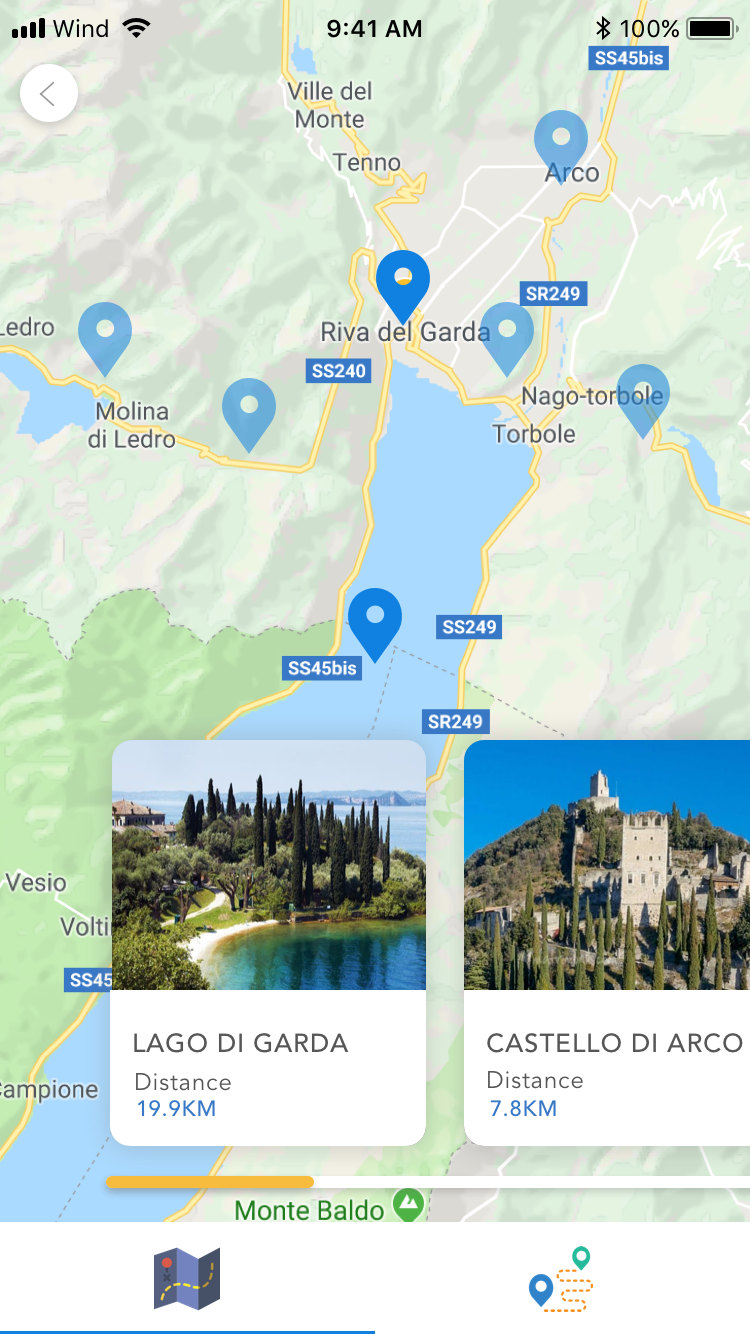
\includegraphics[width=0.3\textwidth]{images/listapunti.png}
\caption{Confronto HomeScreen Open Air Museum vecchia e nuova versione}
\end{figure}
\vspace{5mm}

\begin{figure}[h]
\centering

\includegraphics[width=0.3\textwidth]{images/screenSantarcangelo1.jpg}

\includegraphics[width=0.3\textwidth]{images/singolopunto.png}
\caption{Confronto HomeScreen Open Air Museum vecchia e nuova versione}
\end{figure}
\vspace{5mm}

\begin{figure}[h]
\centering

\includegraphics[width=0.3\textwidth]{images/listapercorsiold.jpg}

\includegraphics[width=0.3\textwidth]{images/listapercorsi.png}
\caption{Confronto HomeScreen Open Air Museum vecchia e nuova versione}
\end{figure}
\vspace{5mm}


Sfruttando la potente libreria di animazioni fornite da React-native è stato possibile creare un'interfaccia ricca e moderna mantenendo le prestazioni elevate anche su dispositivi non recenti e di alta fascia. Il “driver” di tale libreria è infatti nativo ed implementato nel modo più efficiente per i due sistemi operativi. Questo offre solide prestazioni anche nel caso di animazioni molto complesse ma aggiunge anche alcune limitazioni. La più evidente è l’obbligo di implementare tali animazioni con un pattern dichiarativo indicando quindi in precedenza il modo in cui l’oggetto deve comportarsi per poi avere la possibilità di eseguirlo mediante un'interfaccia di start e stop. Tale problematica non ha composto un grave problema implementativo. DI fatto si è trattato solamente di implementare il tutto seguendo il pattern descritto sopra.\vspace{5mm}

Un'ulteriore funzionalità richiesta al porting è quella di poter, riprodurre dei contenuti audio all’interno dell’applicativo. In particolare questi contenuti audio sono presenti sul server e sono serviti attraverso un'api che permette il loro streaming. In precedenza era stato sviluppato un player che utilizzava i rispettivi sdk nativi per controllare l’audio, erano in grado di avviare e stoppare l’audio e proseguire avanti veloce mediante una barra di trascinamento. Le funzionalità per i due sistemi operativi erano le stesse ma viste le diversità tra le due piattaforme è stato necessario re implementare la stessa logica due volte. Utilizzando React-native è stato possibile scrivere la logica una sola volta e condividerla tra le due piattaforme utilizzando un package open source chiamato react-native-audio-streamer. Tale package permette di configurare uno stream audio mediante un url e di controllare la riproduzione, tale libreria utilizza la medesima implementazione attraverso il “bridge” sfruttando a livello nativo due librerie distinte. Per Ios DuoAudioStreamer mentre per Android ExoPlayer. L’utilizzo di tale package accelera lo sviluppo di questa parte mostrando il vantaggio di React-native sopra a soluzioni simili e cioè l’ecosistema. Creare una dipendenza esterna in un progetto enterprise come questo può essere una scelta rischiosa. Legarsi ad un software di terze parti per una features cruciale dell’applicativo può sfociare in problematiche che spaziano dal mantenimento futuro a bug non facilmente tracciabili ma data la semplicità di questa particolare libreria tale rischio è ragionevolmente contenuto.\vspace{5mm}

Come si è visto l’impiego di React-native non ha soppiantato la totalità della parte nativa, anzi questo approccio “misto” ha permesso di non trovarsi limitati da una tecnologia rispetto ad un altra offrendo sempre il giusto tool per la features richiesta. Durante le ricerche legate allo sviluppo di questo prodotto non sono stati trovati linguaggi o framework più flessibili e adatti alle molteplici configurazioni di questo progetto, questo specifico caso è un ottimo esempio di come l’impiego di Javascript al di fuori dal browser sia la scelta vincente per creare un applicativo moderno e flessibile senza sacrificare manutenibilità e consistenza nel tempo.\vspace{5mm}

\section{Punti critici e problematiche}
\vspace{5mm}Durante questo porting sono stati evidenziati una serie di punti critici implementativi, ne discuterò indicando la soluzione da me intrapresa e se presente una soluzione alternativa.\vspace{5mm}

L’utilizzo di una libreria esterna come quella per la gestione degli stream audio oppure quella per gestire la mappa, creano delle dipendenze che aggiungono una serie di incognite sulla longevità del prodotto. E’ importante legare il progetto il meno possibile a risorse esterne non del tutto affidabili. Per tale ragione entrambe le risorse esterne che l’applicativo utilizza e cioè la libreria per lo streaming audio e l’SDK Estimote sono gestite attraverso un layer software. L’applicativo utilizza la libreria attraverso le Api fornite da questa interfaccia, in caso di necessità si può sostituire più agevolmente la vecchia libreria con la nuova mappando le nuove api sull’interfaccia. Ovviamente questo è possibile nei limiti di una coesione logica tra la il vecchio e nuovo SDK. Da notare che un'implementazione di questo tipo permette inoltre di abbandonare del tutto il software esterno implementando la propria libreria integrandola nel progetto facilmente attraverso tale interfaccia. Un ulteriore possibile soluzione a questo problema sarebbe quello di gestire internamente la maggior parte del software ma in alcuni casi questa soluzione deve essere scartata per l’elevato costo.\vspace{5mm}

Altra problematica è data dalla coesistenza di tre linguaggi differenti nella stessa codebase. In alcuni casi React-native può aggiungere complessità invece che rimuoverla, infatti se la quantità di codice nativo a cui dover attingere è molto grande si rischia di dover mantenere tre ecosistemi a differenza di due. Maggiori sono le tecnologie da conoscere per operare su di un prodotto maggiore è il bagaglio necessario per mantenerlo, questo rende il software più complesso da gestire. In questo caso un'attenta analisi del progetto prima dello sviluppo può guidare verso una soluzione differente ed evitare il problema. Nel caso specifico la quantità di codice nativo necessaria non è stata molta ma tale problema potrà presentarsi in futuro con il proseguire del progetto.\vspace{5mm}

Un alto punto critico da mantenere in considerazione con questo tipo di porting è la completa scomparse di database Sql in favore di uno state manager ad oggetti. Data l'impossibilità di gestire i dati in modo paritetico rispetto alla versione nativa è stato necessario riadattare la logica applicativa a questa nuova tecnologia. Non esistendo più tempi di latenza per accedere ai dati questo ha migliorato molto la pulizia e l'asciuttezza del codice. La modifica dei dati avviene attraverso mutazioni allo stato e questo comporta in caso di applicativi molto grandi una crescente complessità se non si dividono in modo accorto le varie aree dello stato dividendo in modo netto una area dall'altra usando nodi il più possibile vicini alla radice. Tale approccio infatti permette di ottenere una buona "separation of concerns"\cite{SOC} delle varie aree logiche dell'applicativo ponendo entrypoint diversi per l'accesso ai dati a seconda della zona logica prestabilita. Ciò permette di risolvere il problema descritto sopra, offrendo un guadagno in termini di semplicità rispetto ad una soluzione basata su SqLite.

